
	\subsection{Variational Monte Carlo calculations of the helium atom}
		As a first attempt to solve the ground state energy for the helium
		atom we perform Variational Monte Carlo calculation with a brute force
		Metropolis sampling. We do this with two trial wave functions
		\[
		\psi_{T}({\bf r_{1}},{\bf r_{2}},{\bf r_{12}})=\exp{\left(-\alpha(r_{1}+r_{2})\right)}\exp{\left(\frac{r_{12}}{2(1+\beta r_{12})}\right)},
		\]
		using $\alpha$ and $\beta$ as variational parameters. 
		We run the Variational Monte Carlo calculation over
		different values for the two variables $\alpha$ and $\beta$, 
		with $2\times10^{7}$ cycles in the Monte Carlo simulation, we get the results
		presented in figure \ref{fig:HeliumAlphaBeta}.
		
		We find the optimal values to be  $\alpha=1.843$ and $\beta=0.34$, as we can see in the figures.
		Using these values for $\alpha$ and $\beta$ we run the brute force variational Monte Carlo calculation. The program finds an optimal value for the steplength, $\delta$, which results in roughly 50\% accepted moves. Using $10^{8}$ cycles the algorithm finds the steplength to be $\delta = 1.5$, giving 48.8\% accepted moves. The energy found with this method is $-2.89024$ au, with a variance of $3.77402\times10^{-5}$, as presented in table \ref{tab:Helium_no_IS}.
		The parameter $\alpha$ can be interpreted as a parameter for the
		force pulling the electron to the nucleus.

		\begin{table}
			\center
			\begin{tabular}{|c|c|c|c|c|c|c|}
			    \hline
			   	Atom  & $\alpha$ & $\beta$ & Cycles & VMC {[}au{]} & Variance & Reference energy {[}au{]} \tabularnewline
				\hline 
				Helium & $1.843$ & $0.34$ & $10^{8}$ & $-2.89024$ & $3.77402\times10^{-5}$ & $-2.9037$\tabularnewline
				\hline 
			\end{tabular}
			\caption{Comparison of the energy for Helium found with VMC without using Importance Sampling, and the reference energy found in research papers \parencite{Binkley_1975}.}
			\label{tab:Helium_no_IS}
		\end{table}
		


		\begin{figure}
			\centering 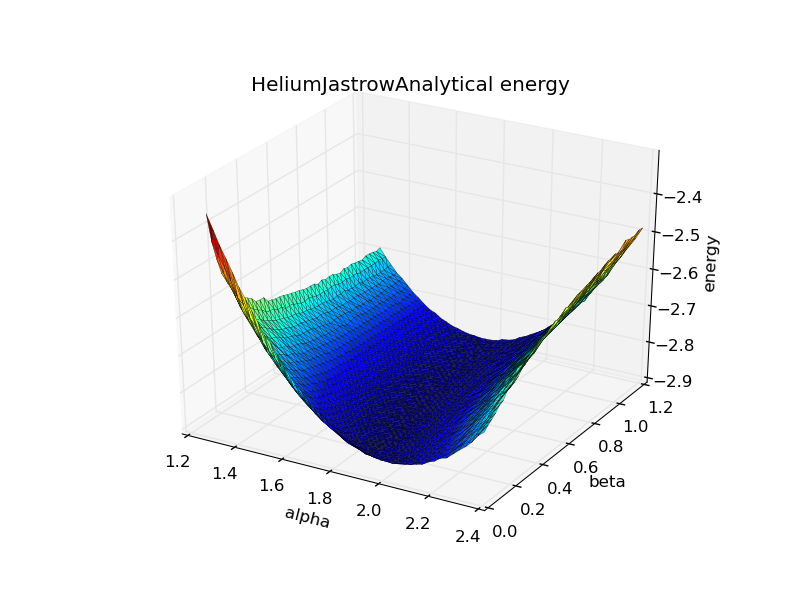
\includegraphics[width=0.49\linewidth]{../figures/HeliumJastrowAnalytical_alpha_beta_energy}
			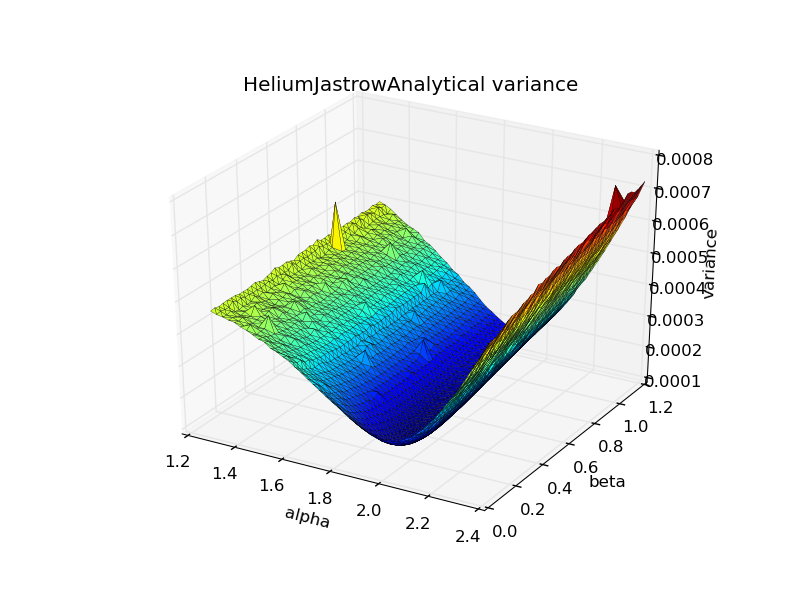
\includegraphics[width=0.49\linewidth]{../figures/HeliumJastrowAnalytical_alpha_beta_variance}
			\protect\caption{Using $\psi_{T}$, plot of the energy versus alpha and beta, and plot of the variance versus $\alpha$ and $\beta$. }
			\label{fig:HeliumAlphaBeta}
		\end{figure}


		\subsubsection{Alpha and Beta Values}

			Table \ref{tab:EnergyAlphaBetaReference} shows the values, for \(\alpha\) and \(\beta\) values, we got from  running several Monte Carlo cycles with different values. As an algorithm to pick out the best values we minimized the energy found in the Monte Carlo runs. The values found are quite uncertain since the variance of the energy was quite high compared to the difference caused by varying the parameters. The variance was more smooth as a function of the parameters, see fig \ref{fig:HeliumAlphaBeta} and it is therefore easier to determine the best values for the variables from variance as a function of \(\alpha\) and \(\beta\).




		\subsubsection{Computational speed gain by using an analytical local energy}
			By using an analytical expression for the local energy instead of using a numerical derivation in the calculation the program becomes more efficient. For Helium we get a speedup of nearly 48\%, while for Beryllium we get a speedup of approximately 80\% was achieved, see table \ref{tab:analyticVSNumeric}.

			\begin{table}
				\center
				\begin{tabular}{| c | c | c | c |}
				    \hline
				   	\textbf{Trialfunction} & Numerical (s) & Analytical (s) & Ratio
				    \\ \hline
				    Helium $\psi_{T}$ & 29.7288 & 20.1189	& 0.6767
				    \\	\hline
				    Beryllium $\psi_{T2}$ & 58.9623  &	32.4622 & 0.5505
					    \\ \hline
				\end{tabular}
				\caption{The time to run a Monte Carlo run with \(10^7\) cycles for Helium, and \(10^6\) cycles for Beryllium. The closed expression for the local energy increased the computation time by a significant degree for each trialfunction. }
				\label{tab:analyticVSNumeric}
			\end{table}

		\subsubsection{Calculations using importance sampling}
			We now introduce importance sampling to our calculations. We search for the optimal variables and find them to be $\alpha=1.843$ and $\beta=0.34$. Using these values, with $10^{8}$ cycles, we get an energy of $-2.89012$ au and a corresponding variance $7.76888\times10^{-5}$, as presented in table \ref{tab:EnergyAlphaBetaReference}. The energy and variance as a function of the timestep, $\delta t$ is shown in figure \ref{fig:HeliumTimestep}.

			\begin{figure}
				\centering 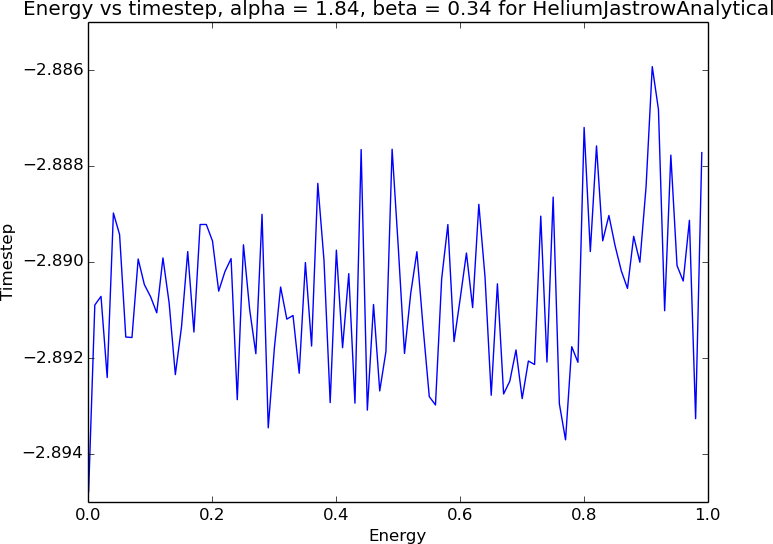
\includegraphics[width=0.45\linewidth]{../figures/HeliumJastrowAnalyticalTimeEnergy}
				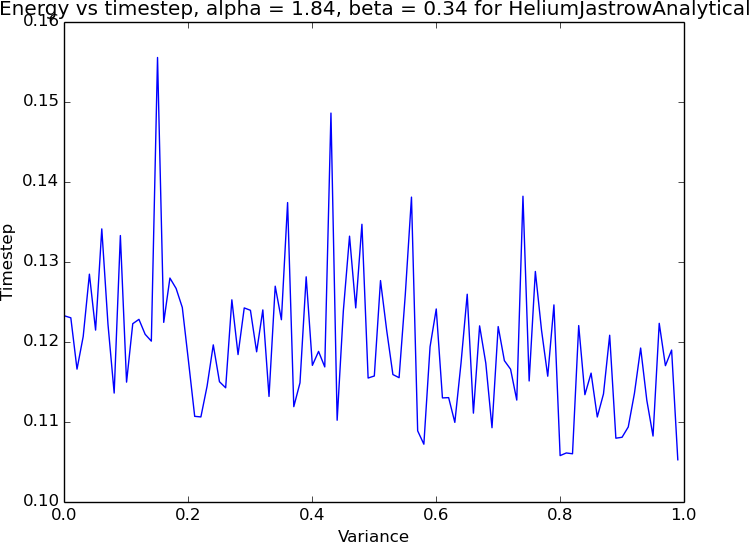
\includegraphics[width=0.45\linewidth]{../figures/HeliumJastrowAnalyticalTimeVariance}
				\protect\caption{Plots for Helium $\psi_{T}$ for the energy versus the timestep, and the variance versus the timestep.}
				\label{fig:HeliumTimestep}
			\end{figure}

			\begin{figure}
				\centering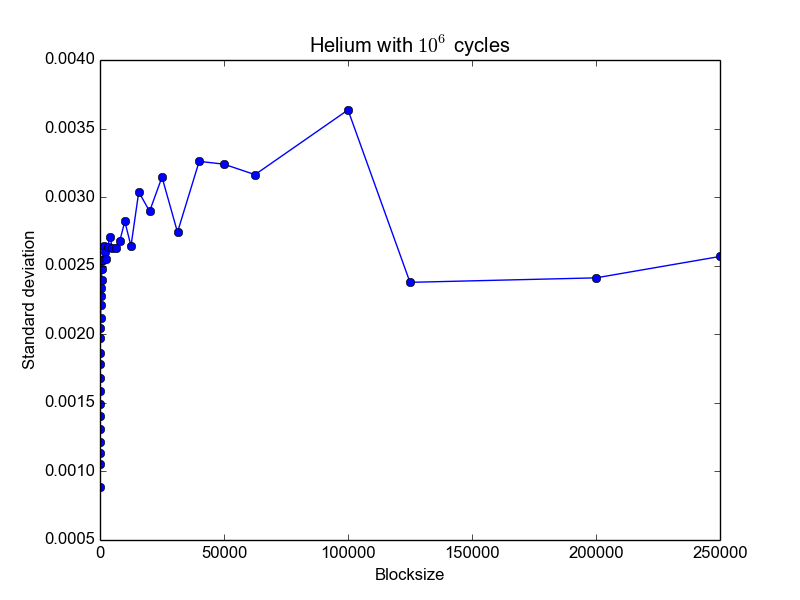
\includegraphics[width=0.45\linewidth]{../figures/Helium_blocking}
				\protect\caption{Variance vs. blocksize for Helium. The blocking behaviour can be seen very clearly as the variance plateaus as the blocksize grows.}
				\label{fig:HeliumBlocking}
			\end{figure}


		\subsubsection{Bisection method and GTOs}

		Using GTOs we can nearly reproduce the energies we get from using Slater Type Orbitals, although we are unable to reach quite the same energy. This is due to the GTOs being an imperfect representation of the STOs. Using GTOs in stead of STOs is also considerably slower, as we see in \ref{tab:AtomsGTO}. This can be due to inefficient code, and there is also room for improvements by calculating analytical derivatives of the GTOs. However using GTOs reduces the variables to only $\beta$, thus we don't have to look for energy minima by varying $\alpha$. This means that it is possible to easily use a gradient method to more efficiently find the variable that gives minimum energy.
